\documentclass[]{tufte-book}

% ams
\usepackage{amssymb,amsmath}

\usepackage{ifxetex,ifluatex}
\usepackage{fixltx2e} % provides \textsubscript
\ifnum 0\ifxetex 1\fi\ifluatex 1\fi=0 % if pdftex
  \usepackage[T1]{fontenc}
  \usepackage[utf8]{inputenc}
\else % if luatex or xelatex
  \makeatletter
  \@ifpackageloaded{fontspec}{}{\usepackage{fontspec}}
  \makeatother
  \defaultfontfeatures{Ligatures=TeX,Scale=MatchLowercase}
  \makeatletter
  \@ifpackageloaded{soul}{
     \renewcommand\allcapsspacing[1]{{\addfontfeature{LetterSpace=15}#1}}
     \renewcommand\smallcapsspacing[1]{{\addfontfeature{LetterSpace=10}#1}}
   }{}
  \makeatother

\fi

% graphix
\usepackage{graphicx}
\setkeys{Gin}{width=\linewidth,totalheight=\textheight,keepaspectratio}

% booktabs
\usepackage{booktabs}

% url
\usepackage{url}

% hyperref
\usepackage{hyperref}

% units.
\usepackage{units}


\setcounter{secnumdepth}{2}

% citations
\usepackage{natbib}
\bibliographystyle{apalike}

% pandoc syntax highlighting

% longtable
\usepackage{longtable,booktabs}

% multiplecol
\usepackage{multicol}

% strikeout
\usepackage[normalem]{ulem}

% morefloats
\usepackage{morefloats}


% tightlist macro required by pandoc >= 1.14
\providecommand{\tightlist}{%
  \setlength{\itemsep}{0pt}\setlength{\parskip}{0pt}}

% title / author / date
\title{Improving the Reproducibility of Experimental Data Recording and Pre-Processing}
\author{Brooke Anderson, Michael Lyons, Mercedes Gonzalez-Juarrero, Marcela Henao-Tamayo, and Gregory Robertson}
\date{}

\usepackage{booktabs}
\usepackage{amsthm}
\usepackage{fontspec}
    \setmainfont{Gill Sans}
\makeatletter
\def\thm@space@setup{%
  \thm@preskip=8pt plus 2pt minus 4pt
  \thm@postskip=\thm@preskip
}
\makeatother

\begin{document}

\maketitle



{
\setcounter{tocdepth}{1}
\tableofcontents
}

\hypertarget{overview}{%
\chapter{Overview}\label{overview}}

\newthought{The recent NIH-Wide Strategic Plan} \citep{nih2016strategic}
describes an integrative view of biology and human health that includes
translational medicine, team science, and the importance of capitalizing on an
exponentially growing and increasingly complex data ecosystem \citep{nih2018data}.
Underlying this view is the need to use, share, and re-use biomedical data
generated from widely varying experimental systems and researchers. Basic
sources of biomedical data range from relatively small sets of measurements,
such as animal body weights and bacterial cell counts that may be recorded by
hand, to thousands or millions of instrument-generated data points from various
imaging, -omic, and flow cytometry experiments. In either case, there is a
generally common workflow that proceeds from measurement to data recording,
pre-processing, analysis, and interpretation. However, in practice the distinct
actions of data recording, data pre-processing, and data analysis are often
merged or combined as a single entity by the researcher using commercial or open
source spreadsheets, or as part of an often proprietary experimental measurement
system / software combination (Figure \ref{fig:workflow}), resulting in key
failure points for reproducibility at the stages of data recording and
pre-processing.

\begin{figure*}

{\centering 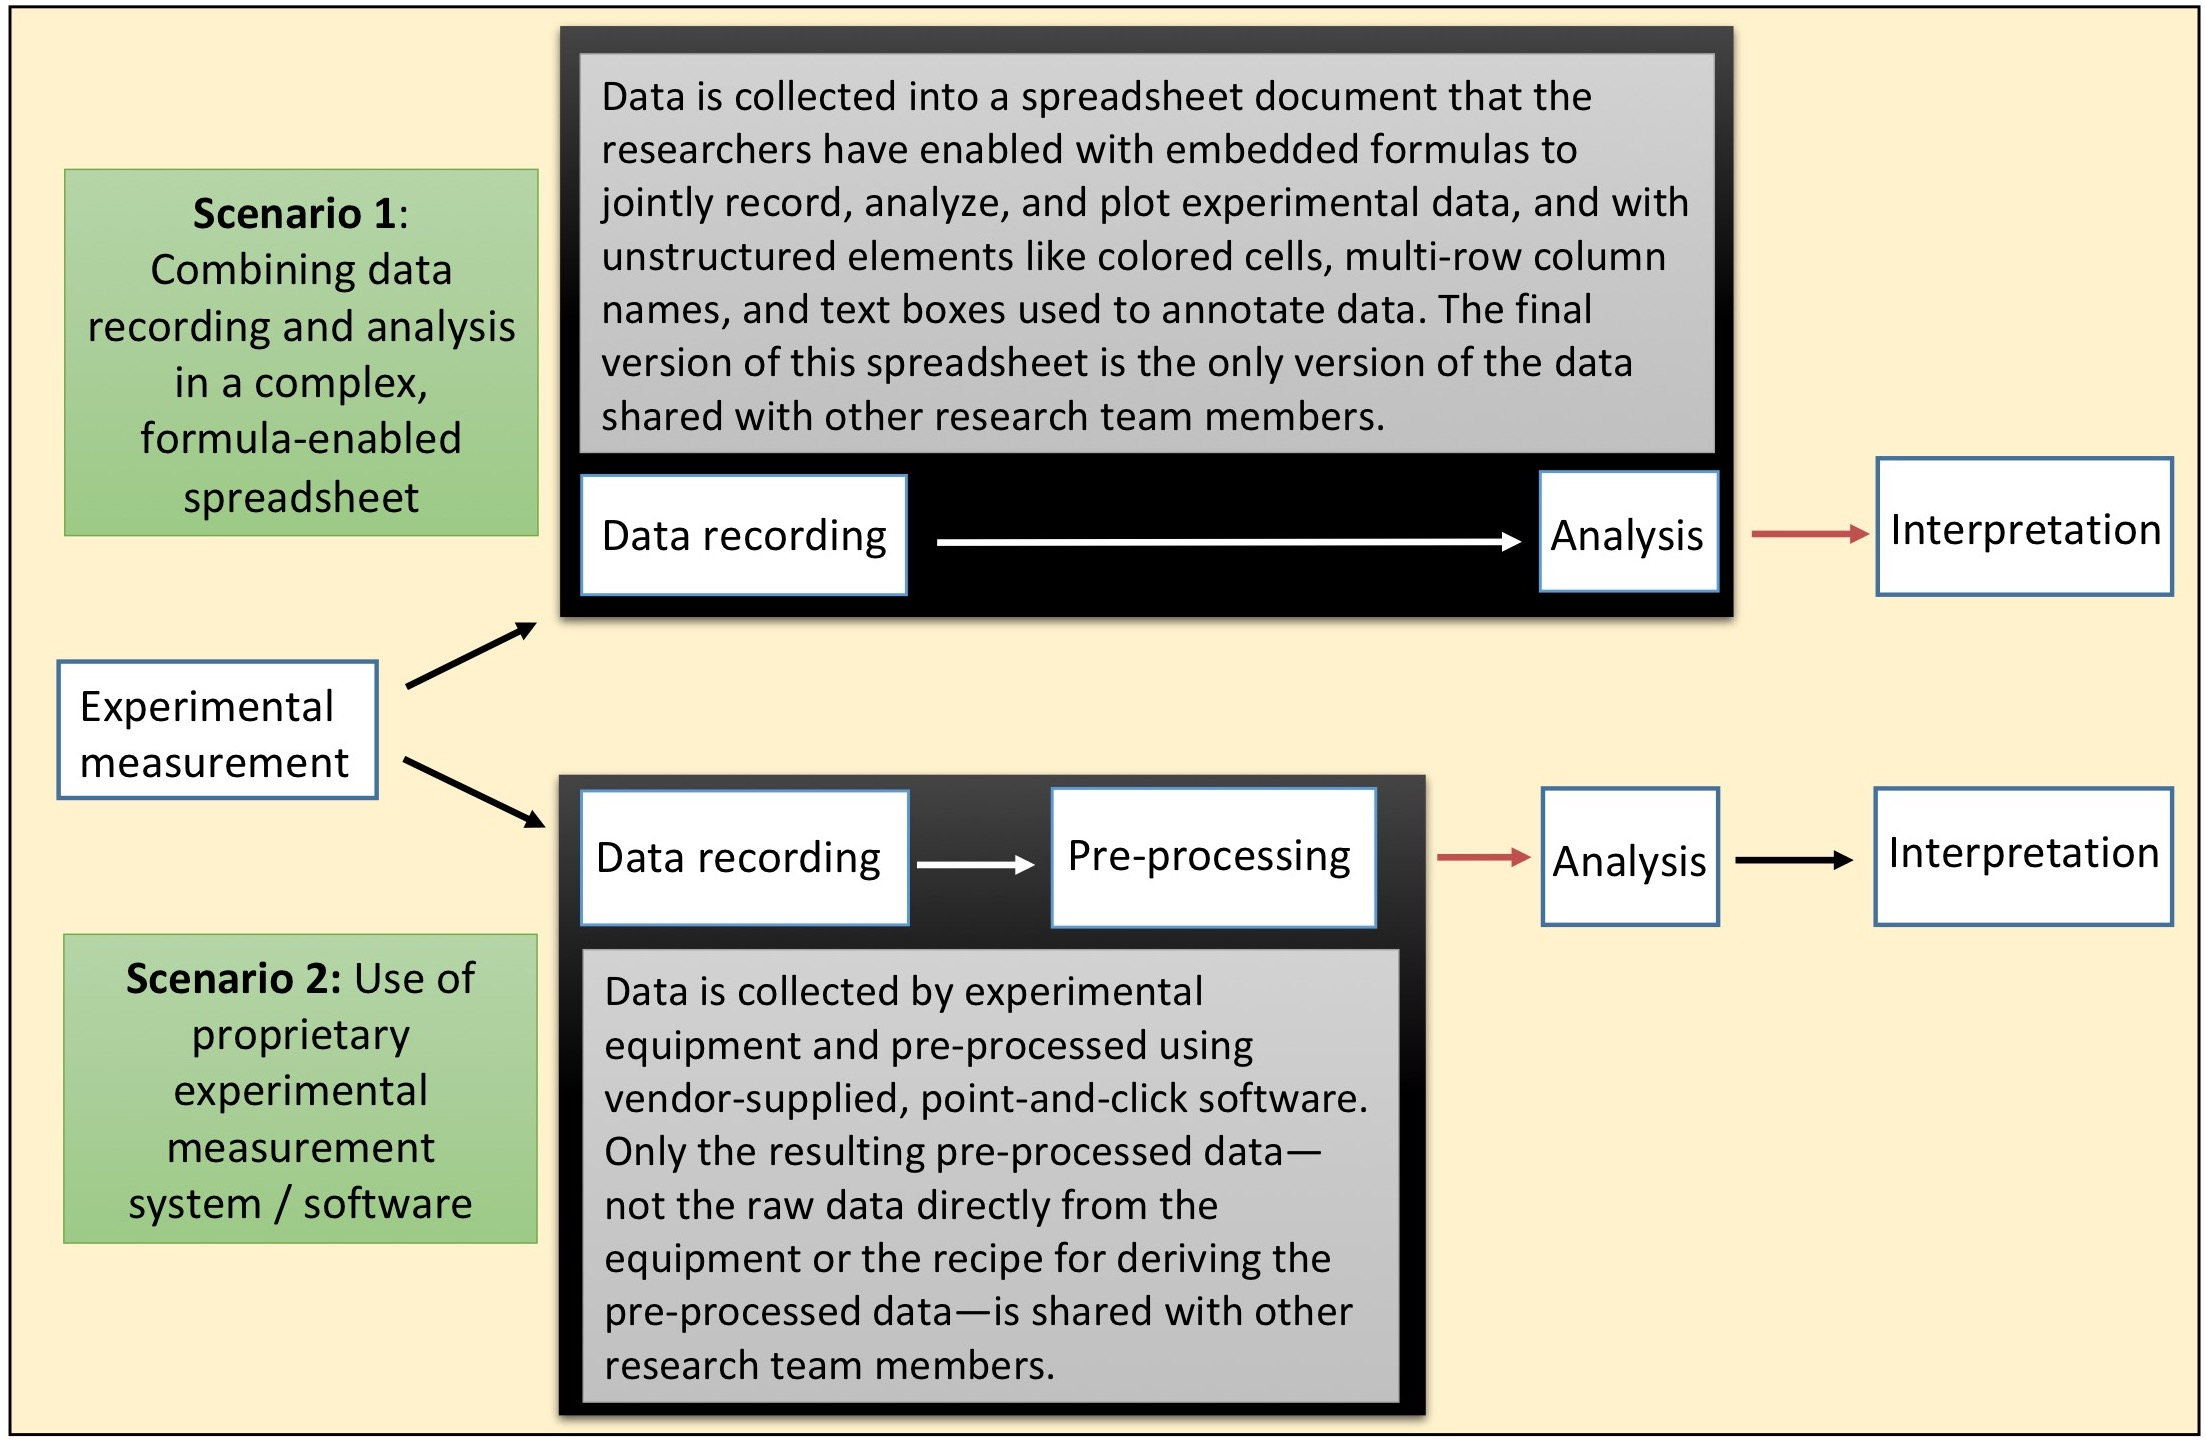
\includegraphics[width=30.64in]{figures/existing_blackboxes} 

}

\caption[Two scenarios where 'black boxes' of non-transparent, non-reproducible data handling exist in research data workflows at the stages of data recording and pre-processing]{Two scenarios where 'black boxes' of non-transparent, non-reproducible data handling exist in research data workflows at the stages of data recording and pre-processing. These create potential points of failure for reproducible research. Red arrows indicate where data is passed to other research team members, including statisticians / data analysts, often within complex or unstructured spreadsheet files.}\label{fig:workflow}
\end{figure*}

It is widely known and discussed among data scientists, mathematical modelers,
and statisticians \citep{broman2018data, krishnan2016towards} that there is
frequently a need to discard, transform, and reformat various elements of the
data shared with them by laboratory-based researchers, and that data is often
shared in an unstructured format, increasing the risks of introducing errors
through reformatting before applying more advanced computational methods.
Instead, a critical need for reproducibility is for the transparent and clear
sharing across research teams of: (1) raw data, directly from hand-recording or
directly output from experimental equipment; (2) data that has been
pre-processed as necessary (e.g., gating for flow cytometry data, feature
identification for metabolomics data), saved in a consistent, structured format,
and (3) a clear and repeatable description of how the pre-processed data was
generated from the raw data \citep{broman2018data, ellis2018share}.

To enhance data reproducibility, it is critical to create a clear separation
among data recording, data pre-processing, and data analysis---breaking up
commonly existing ``black boxes" in data handling across the research process.
Such a rigorous demarcation requires some change in the conventional
understanding and use of spreadsheets and a recognition by biomedical
researchers that recent advances in computer programming languages, especially
the R programming language, provide user-friendly and accessible tools and
concepts that can be used to extend a transparent and reproducible data workflow
to the steps of data recording and pre-processing. Among our team, we have found
that there are many common existing practices---including use of spreadsheets
with embedded formulas that concurrently record and analyze experimental data,
problematic management of project files, and reliance on proprietary,
vendor-supplied point-and-click software for data pre-processing---that can
interfere with the transparency, reproducibility, and efficiency of
laboratory-based biomedical research projects, problems that have also been
identified by others as key barriers to research reproducibility
\citep[ \citet{marwick2018packaging}]{broman2018data, bryan2018excuse, ellis2018share}. In
these training modules, we have choosen topics that tackle barriers to
reproducibility that have straightforward, easy-to-teach solutions, but which
are still very common in biomedical laboratory-based research programs.

\hypertarget{license}{%
\section{License}\label{license}}

This book is licensed under the \href{https://creativecommons.org/licenses/by-nc-sa/4.0/}{Creative Commons
Attribution-NonCommercial-ShareAlike 4.0 International
License}, while all code in
the book is under the \href{https://opensource.org/licenses/MIT}{MIT license}.

Click on the \textbf{Next} button (or navigate using the
links at the top of the page) to continue.

\hypertarget{experimental-data-recording}{%
\chapter{Experimental Data Recording}\label{experimental-data-recording}}

\hypertarget{separating-data-recording-and-analysis}{%
\section{Separating data recording and analysis}\label{separating-data-recording-and-analysis}}

Many biomedical laboratories use spreadsheets, with embedded formulas, to both
record and analyze experimental data. This practice impedes transparency and
reproducibility of both data recording and data analysis. In this module, we
will describe this common practice and will outline alternative approaches that
separate the steps of data recording and data analysis.

\textbf{Objectives.} After this module, the trainee will be able to:

\begin{itemize}
\tightlist
\item
  Explain the difference between data recording and data analysis
\item
  Understand why collecting data on spreadsheets with embedded formulas impedes
  reproducibility
\item
  List alternative approaches to improve reproducibility
\end{itemize}

\hypertarget{data-recording-versus-data-analysis}{%
\subsection{Data recording versus data analysis}\label{data-recording-versus-data-analysis}}

\hypertarget{common-practices-combining-recording-and-analysis}{%
\subsection{Common practices combining recording and analysis}\label{common-practices-combining-recording-and-analysis}}

\hypertarget{hazards-of-combining-recording-and-analysis}{%
\subsection{Hazards of combining recording and analysis}\label{hazards-of-combining-recording-and-analysis}}

\hypertarget{approaches-to-separate-recording-and-analysis}{%
\subsection{Approaches to separate recording and analysis}\label{approaches-to-separate-recording-and-analysis}}

\hypertarget{discussion-questions}{%
\subsection{Discussion questions}\label{discussion-questions}}

\hypertarget{principles-and-power-of-structured-data-formats}{%
\section{Principles and power of structured data formats}\label{principles-and-power-of-structured-data-formats}}

The format in which experimental data is recorded can have a large influence on
how easy and likely it is to implement reproducibility tools in later stages of
the research workflow. Recording data in a ``structured'' format brings many
benefits. In this module, we will explain what makes a dataset ``structured'' and
why this format is a powerful tool for reproducible research.

\textbf{Objectives.} After this module, the trainee will be able to:

\begin{itemize}
\tightlist
\item
  List the characteristics of a structured data format
\item
  Describe benefits for research transparency and reproducibility
\item
  Outline other benefits of using a structured format when recording data
\end{itemize}

\hypertarget{characteristics-of-a-structured-data-format}{%
\subsection{Characteristics of a structured data format}\label{characteristics-of-a-structured-data-format}}

\hypertarget{benefits-of-a-structured-data-format}{%
\subsection{Benefits of a structured data format}\label{benefits-of-a-structured-data-format}}

\hypertarget{applied-exercise}{%
\subsection{Applied exercise}\label{applied-exercise}}

\hypertarget{the-tidy-data-format}{%
\section{The `tidy' data format}\label{the-tidy-data-format}}

The ``tidy'' data format is an implementation of a structured data format popular
among statisticians and data scientists. By consistently using this data format,
researchers can combine simple, generalizable tools to perform complex tasks in
data processing, analysis, and visualization. We will explain what
characteristics determine if a dataset is ``tidy'' and how use of the ``tidy''
implementation of a structure data format can improve the ease and efficiency of
``Team Science''.

\textbf{Objectives.} After this module, the trainee will be able to:

\begin{itemize}
\tightlist
\item
  List characteristics defining the ``tidy'' structured data format
\item
  Explain the difference between the a structured data format (general concept)
  and the `tidy' data format (one popular implementation)
\end{itemize}

\hypertarget{the-tidy-data-format-1}{%
\subsection{The ``tidy'' data format}\label{the-tidy-data-format-1}}

\hypertarget{the-tidy-data-format-as-a-structured-data-format}{%
\subsection{The ``tidy'' data format as a structured data format}\label{the-tidy-data-format-as-a-structured-data-format}}

\hypertarget{practice-quiz}{%
\subsection{Practice quiz}\label{practice-quiz}}

\hypertarget{designing-templates-for-tidy-data-collection}{%
\section{Designing templates for ``tidy'' data collection}\label{designing-templates-for-tidy-data-collection}}

This module will move from the principles of the ``tidy'' data format to the
practical details of designing a ``tidy'' data format to use when collecting
experimental data. We will describe common issues that prevent biomedical
research datasets from being ``tidy'' and show how these issues can be avoided. We
will also provide rubrics and a checklist to help determine if a data collection
template complies with a ``tidy'' format.

\textbf{Objectives.} After this module, the trainee will be able to:

\begin{itemize}
\tightlist
\item
  Identify characteristics that keep a dataset from being `tidy'
\item
  Convert data from an ``untidy'' to a ``tidy'' format
\end{itemize}

\hypertarget{subsection-1}{%
\subsection{Subsection 1}\label{subsection-1}}

\hypertarget{applied-exercise-1}{%
\subsection{Applied exercise}\label{applied-exercise-1}}

\hypertarget{example-creating-a-template-for-tidy-data-collection}{%
\section{Example: Creating a template for ``tidy'' data collection}\label{example-creating-a-template-for-tidy-data-collection}}

We will walk through an example of creating a template to collect data in a
``tidy'' format for a laboratory-based research project, based on a research
project on drug efficacy in murine tuberculosis models. We will show the initial
``untidy'' format for data recording and show how we converted it to a ``tidy''
format. Finally, we will show how the data can then easily be analyzed and
visualized using reproducible tools.

\textbf{Objectives.} After this module, the trainee will be able to:

\begin{itemize}
\tightlist
\item
  Understand how the principles of ``tidy'' data can be applied for a real, complex research project;
\item
  List advantages of the ``tidy'' data format for the example project
\end{itemize}

\hypertarget{subsection-1-1}{%
\subsection{Subsection 1}\label{subsection-1-1}}

\hypertarget{subsection-2}{%
\subsection{Subsection 2}\label{subsection-2}}

\hypertarget{discussion-questions-1}{%
\subsection{Discussion questions}\label{discussion-questions-1}}

\hypertarget{power-of-using-a-single-structured-project-directory-for-storing-and-tracking-research-project-files}{%
\section{Power of using a single structured `Project' directory for storing and tracking research project files}\label{power-of-using-a-single-structured-project-directory-for-storing-and-tracking-research-project-files}}

To improve the computational reproducibility of a research project, researchers
can use a single `Project' directory to collectively store all research data,
meta-data, pre-processing code, and research products (e.g., paper drafts,
figures). We will explain how this practice improves the reproducibility and
list some of the common components and subdirectories to include in the
structure of a `Project' directory, including subdirectories for raw and
pre-processed experimental data.

\textbf{Objectives.} After this module, the trainee will be able to:

\begin{itemize}
\tightlist
\item
  Describe a `Project' directory, including common components and subdirectories
\item
  List how a single `Project' directory improves reproducibility
\end{itemize}

\hypertarget{subsection-1-2}{%
\subsection{Subsection 1}\label{subsection-1-2}}

\hypertarget{subsection-2-1}{%
\subsection{Subsection 2}\label{subsection-2-1}}

\hypertarget{practice-quiz-1}{%
\subsection{Practice quiz}\label{practice-quiz-1}}

\hypertarget{creating-project-templates}{%
\section{Creating `Project' templates}\label{creating-project-templates}}

Researchers can use RStudio's `Projects' can facilitate collecting research
files in a single, structured directory, with the added benefit of easy use of
version control. Researchers can gain even more benefits by consistently
structuring all their `Project' directories. We will demonstrate how to
implement structured project directories through RStudio, as well as how RStudio
enables the creation of a `Project' for initializing consistently-structured
directories for all of a research group's projects.

\textbf{Objectives.} After this module, the trainee will be able to:

\begin{itemize}
\tightlist
\item
  Be able to create a structured \texttt{Project} directory within RStudio
\item
  Understand how RStudio can be used to create `Project' templates
\end{itemize}

\hypertarget{subsection-1-3}{%
\subsection{Subsection 1}\label{subsection-1-3}}

\hypertarget{subsection-2-2}{%
\subsection{Subsection 2}\label{subsection-2-2}}

\hypertarget{discussion-questions-2}{%
\subsection{Discussion questions}\label{discussion-questions-2}}

\hypertarget{example-creating-a-project-template}{%
\section{Example: Creating a `Project' template}\label{example-creating-a-project-template}}

We will walk through a real example, based on the experiences of one of our
Co-Is, of establishing the format for a research group's `Project' template,
creating that template using RStudio, and initializing a new research project
directory using the created template. This example will be from a
laboratory-based research group that studies the efficacy of tuberculosis drugs
in a murine model.

\textbf{Objectives.} After this module, the trainee will be able to:

\begin{itemize}
\tightlist
\item
  Create a `Project' template in RStudio to initialize consistently-formatted
  `Project' directories
\item
  Initialize a new `Project' directory using this template
\end{itemize}

\hypertarget{subsection-1-4}{%
\subsection{Subsection 1}\label{subsection-1-4}}

\hypertarget{subsection-2-3}{%
\subsection{Subsection 2}\label{subsection-2-3}}

\hypertarget{applied-exercise-2}{%
\subsection{Applied exercise}\label{applied-exercise-2}}

\hypertarget{harnessing-version-control-for-transparent-data-recording}{%
\section{Harnessing version control for transparent data recording}\label{harnessing-version-control-for-transparent-data-recording}}

As a research project progresses, a typical practice in many experimental
research groups is to save new versions of files (e.g., `draft1.doc',
`draft2.doc'), so that changes can be reverted. However, this practice leads to
an explosion of files, and it becomes hard to track which files represent the
`current' state of a project. Version control allows researchers to edit and
change research project files more cleanly, while maintaining the power to
`backtrack' to previous versions, messages included to explain changes. We will
explain what version control is and how it can be used in research projects to
improve the transparency and reproducibility of research, particularly for data
recording.

\textbf{Objectives.} After this module, the trainee will be able to:

\begin{itemize}
\tightlist
\item
  Describe version control\\
\item
  Explain how version control can be used to improve reproducibility
  for data recording
\end{itemize}

\hypertarget{subsection-1-5}{%
\subsection{Subsection 1}\label{subsection-1-5}}

\hypertarget{subsection-2-4}{%
\subsection{Subsection 2}\label{subsection-2-4}}

\hypertarget{discussion-questions-3}{%
\subsection{Discussion questions}\label{discussion-questions-3}}

\hypertarget{enhance-the-reproducibility-of-collaborative-research-with-version-control-platforms}{%
\section{Enhance the reproducibility of collaborative research with version control platforms}\label{enhance-the-reproducibility-of-collaborative-research-with-version-control-platforms}}

Once a researcher has learned to use \emph{git} on their own computer for
local version control, they can begin using version control platforms (e.g.,
\emph{GitLab}, \emph{GitHub}) to collaborate with others under version
control. We will describe how a research team can benefit from using a version
control platform to work collaboratively.

\textbf{Objectives.} After this module, the trainee will be able to:

\begin{itemize}
\tightlist
\item
  List benefits of using a version control platform to collaborate
  on research projects, particularly for reproducibility
\item
  Describe the difference between version control (e.g., \emph{git}) and
  a version control platform (e.g., \emph{GitLab})
\end{itemize}

\hypertarget{subsection-1-6}{%
\subsection{Subsection 1}\label{subsection-1-6}}

\hypertarget{subsection-2-5}{%
\subsection{Subsection 2}\label{subsection-2-5}}

\hypertarget{discussion-questions-4}{%
\subsection{Discussion questions}\label{discussion-questions-4}}

\hypertarget{using-git-and-gitlab-to-implement-version-control}{%
\section{Using git and GitLab to implement version control}\label{using-git-and-gitlab-to-implement-version-control}}

For many years, use of version control required use of the command line,
limiting its accessibility to researchers with limited programming experience.
However, graphical interfaces have removed this barrier, and RStudio has
particularly user-friendly tools for implementing version control. In this
module, we will show how to use \emph{git} through RStudio's user-friendly
interface and how to connect from a local computer to \emph{GitLab} through
RStudio.

\textbf{Objectives.} After this module, the trainee will be able to:

\begin{itemize}
\tightlist
\item
  Understand how to set up and use \emph{git} through RStudio's interface
\item
  Understand how to connect with \emph{GitLab} through RStudio to collaborate on\\
  research projects while maintaining version control
\end{itemize}

\hypertarget{subsection-1-7}{%
\subsection{Subsection 1}\label{subsection-1-7}}

\hypertarget{subsection-2-6}{%
\subsection{Subsection 2}\label{subsection-2-6}}

\hypertarget{applied-exercise-3}{%
\subsection{Applied exercise}\label{applied-exercise-3}}

\hypertarget{experimental-data-preprocessing}{%
\chapter{Experimental Data Preprocessing}\label{experimental-data-preprocessing}}

\hypertarget{principles-and-benefits-of-scripted-pre-processing-of-experimental-data}{%
\section{Principles and benefits of scripted pre-processing of experimental data}\label{principles-and-benefits-of-scripted-pre-processing-of-experimental-data}}

The experimental data collected for biomedical research often requires
pre-processing before it can be analyzed (e.g., gating of flow cytometry data,
feature finding / quantification for mass spectrometry data). Use of
point-and-click software can limit the transparency and reproducibility of this
analysis stage and is time-consuming for repeated tasks. We will explain how
scripted pre-processing, especially using open source software, can improve
transparency and reproducibility.

\textbf{Objectives.} After this module, the trainee will be able to:

\begin{itemize}
\tightlist
\item
  Define `pre-processing' of experimental data
\item
  Describe an open source code script and explain how it can increase
  reproducibility of data pre-processing
\end{itemize}

\hypertarget{subsection-1-8}{%
\subsection{Subsection 1}\label{subsection-1-8}}

\hypertarget{subsection-2-7}{%
\subsection{Subsection 2}\label{subsection-2-7}}

\hypertarget{discussion-questions-5}{%
\subsection{Discussion questions}\label{discussion-questions-5}}

\hypertarget{introduction-to-scripted-data-pre-processing-in-r}{%
\section{Introduction to scripted data pre-processing in R}\label{introduction-to-scripted-data-pre-processing-in-r}}

We will show how to implement scripted pre-processing of experimental data
through R scripts. We will demonstrate the difference between interactive coding
and code scripts, using R for examples. We will then demonstrate how to create,
save, and run an R code script for a simple data cleaning task.

\textbf{Objectives.} After this module, the trainee will be able to:

\begin{itemize}
\tightlist
\item
  Describe what an R code script is and how it differs from interactive
  coding in R
\item
  Create and save an R script to perform a simple data pre-processing task
\item
  Run an R script
\item
  List some popular packages in R for pre-processing biomedical data
\end{itemize}

\hypertarget{subsection-1-9}{%
\subsection{Subsection 1}\label{subsection-1-9}}

\hypertarget{subsection-2-8}{%
\subsection{Subsection 2}\label{subsection-2-8}}

\hypertarget{applied-exercise-4}{%
\subsection{Applied exercise}\label{applied-exercise-4}}

\hypertarget{simplify-scripted-pre-processing-through-rs-tidyverse-tools}{%
\section{Simplify scripted pre-processing through R's `tidyverse' tools}\label{simplify-scripted-pre-processing-through-rs-tidyverse-tools}}

The R programming language now includes a collection of `tidyverse' extension
packages that enable user-friendly yet powerful work with experimental data,
including pre-processing and exploratory visualizations. The principle behind
the `tidyverse' is that a collection of simple, general tools can be joined
together to solve complex problems, as long as a consistent format is used for
the input and output of each tool (the `tidy' data format taught in other
modules). In this module, we will explain why this `tidyverse' system is so
powerful and how it can be leveraged within biomedical research, especially for
reproducibly pre-processing experimental data.

\textbf{Objectives.} After this module, the trainee will be able to:

\begin{itemize}
\tightlist
\item
  Define R's `tidyverse' system
\item
  Explain how the `tidyverse' collection of packages can be both user-friendly
  and powerful in solving many complex tasks with data
\item
  Describe the difference between base R and R's `tidyverse'.
\end{itemize}

\hypertarget{subsection-1-10}{%
\subsection{Subsection 1}\label{subsection-1-10}}

\hypertarget{subsection-2-9}{%
\subsection{Subsection 2}\label{subsection-2-9}}

\hypertarget{practice-quiz-2}{%
\subsection{Practice quiz}\label{practice-quiz-2}}

\hypertarget{complex-data-types-in-experimental-data-pre-processing}{%
\section{Complex data types in experimental data pre-processing}\label{complex-data-types-in-experimental-data-pre-processing}}

Raw data from many biomedical experiments, especially those that use
high-throughput techniques, can be very large and complex. Because of the scale
and complexity of these data, software for pre-processing the data in R often
uses complex, `untidy' data formats. While these formats are necessary for
computational efficiency, they add a critical barrier for researchers wishing to
implement reproducibility tools. In this module, we will explain why use of
complex data formats is often necessary within open source pre-processing
software and outline the hurdles created in reproducibility tool use among
laboratory-based scientists.

\textbf{Objectives.} After this module, the trainee will be able to:

\begin{itemize}
\tightlist
\item
  Explain why R software for pre-processing biomedical data often stores
  data in complex, `untidy' formats
\item
  Describe how these complex data formats can create barriers to
  laboratory-based researchers seeking to use reproducibility tools for
  data pre-processing
\end{itemize}

\hypertarget{subsection-1-11}{%
\subsection{Subsection 1}\label{subsection-1-11}}

\hypertarget{subsection-2-10}{%
\subsection{Subsection 2}\label{subsection-2-10}}

\hypertarget{practice-quiz-3}{%
\subsection{Practice quiz}\label{practice-quiz-3}}

\hypertarget{complex-data-types-in-r-and-bioconductor}{%
\section{Complex data types in R and Bioconductor}\label{complex-data-types-in-r-and-bioconductor}}

Many R extension packages for pre-processing experimental data use complex
(rather than `tidy') data formats within their code, and many output data in
complex formats. Very recently, the \emph{broom} and \emph{biobroom} R
packages have been developed to extract a `tidy' dataset from a complex data
format. These tools create a clean, simple connection between the complex data
formats often used in pre-processing experimental data and the `tidy' format
required to use the `tidyverse' tools now taught in many introductory R courses.
In this module, we will describe the `list' data structure, the common backbone
for complex data structures in R and provide tips on how to explore and extract
data stored in R in this format, including through the \emph{broom} and
\emph{biobroom} packages.

\textbf{Objectives.} After this module, the trainee will be able to:

\begin{itemize}
\tightlist
\item
  Describe the structure of R's `list' data format
\item
  Take basic steps to explore and extract data stored in R's complex, list-based
  structures
\item
  Describe what the \emph{broom} and \emph{biobroom} R packages can do
\item
  Explain how converting data to a `tidy' format can improve reproducibility
\end{itemize}

\hypertarget{subsection-1-12}{%
\subsection{Subsection 1}\label{subsection-1-12}}

\hypertarget{subsection-2-11}{%
\subsection{Subsection 2}\label{subsection-2-11}}

\hypertarget{applied-exercise-5}{%
\subsection{Applied exercise}\label{applied-exercise-5}}

\hypertarget{example-converting-from-complex-to-tidy-data-formats}{%
\section{Example: Converting from complex to `tidy' data formats}\label{example-converting-from-complex-to-tidy-data-formats}}

We will provide a detailed example of a case where data pre-processing in R
results in a complex, `untidy' data format. We will walk through an example of
applying automated gating to flow cytometry data. We will demonstrate the
complex initial format of this pre-processed data and then show trainees how a
`tidy' dataset can be extracted and used for further data analysis and
visualization using the popular R `tidyverse' tools. This example will use real
experimental data from one of our Co-Is research on the immunology of
tuberculosis.

\textbf{Objectives.} After this module, the trainee will be able to:

\begin{itemize}
\tightlist
\item
  Describe how tools like \textit{biobroom} were used in this real research
  example to convert from the complex data format from pre-processing to a format
  better for further data analysis and visualization
\item
  Understand how these tools would fit in their own research pipelines
\end{itemize}

\hypertarget{subsection-1-13}{%
\subsection{Subsection 1}\label{subsection-1-13}}

\hypertarget{subsection-2-12}{%
\subsection{Subsection 2}\label{subsection-2-12}}

\hypertarget{applied-exercise-6}{%
\subsection{Applied exercise}\label{applied-exercise-6}}

\hypertarget{introduction-to-reproducible-data-pre-processing-protocols}{%
\section{Introduction to reproducible data pre-processing protocols}\label{introduction-to-reproducible-data-pre-processing-protocols}}

Reproducibility tools can be used to create reproducible data pre-processing
protocols---documents that combine code and text in a `knitted' document, which
can be re-used to ensure data pre-processing is consistent and reproducible
across research projects. In this module, we will describe how reproducible data
pre-processing protocols can improve reproducibility of pre-processing
experimental data, as well as to ensure transparency, consistency, and
reproducibility across the research projects conducted by a research team.

\textbf{Objectives.} After this module, the trainee will be able to:

\begin{itemize}
\tightlist
\item
  Define a `reproducible data pre-processing protocol'
\item
  Explain how such protocols improve reproducibility at the data pre-processing
  phase
\item
  List other benefits, including improving efficiency and consistency of data
  pre-processing
\end{itemize}

\hypertarget{subsection-1-14}{%
\subsection{Subsection 1}\label{subsection-1-14}}

\hypertarget{subsection-2-13}{%
\subsection{Subsection 2}\label{subsection-2-13}}

\hypertarget{discussion-questions-6}{%
\subsection{Discussion questions}\label{discussion-questions-6}}

\hypertarget{rmarkdown-for-creating-reproducible-data-pre-processing-protocols}{%
\section{RMarkdown for creating reproducible data pre-processing protocols}\label{rmarkdown-for-creating-reproducible-data-pre-processing-protocols}}

The R extension package RMarkdown can be used to create documents that combine
code and text in a `knitted' document, and it has become a popular tool for
improving the computational reproducibility and efficiency of the data analysis
stage of research. This tool can also be used earlier in the research process,
however, to improve reproducibility of pre-processing steps. In this module, we
will provide detailed instructions on how to use RMarkdown in RStudio to create
documents that combine code and text. We will show how an RMarkdown document
describing a data pre-processing protocol can be used to efficiently apply the
same data pre-processing steps to different sets of raw data.

\textbf{Objectives.} After this module, the trainee will be able to:

\begin{itemize}
\tightlist
\item
  Define RMarkdown and the documents it can create
\item
  Explain how RMarkdown can be used to improve the reproducibility of research
  projects at the data pre-processing phase
\item
  Create a document in RStudio using
\item
  Apply it to several different datasets with the same format
\end{itemize}

\hypertarget{subsection-1-15}{%
\subsection{Subsection 1}\label{subsection-1-15}}

\hypertarget{subsection-2-14}{%
\subsection{Subsection 2}\label{subsection-2-14}}

\hypertarget{applied-exercise-7}{%
\subsection{Applied exercise}\label{applied-exercise-7}}

\hypertarget{example-creating-a-reproducible-data-pre-processing-protocol}{%
\section{Example: Creating a reproducible data pre-processing protocol}\label{example-creating-a-reproducible-data-pre-processing-protocol}}

We will walk through an example of creating a reproducible protocol for the
automated gating of flow cytometry data for a project on the immunology of
tuberculosis lead by one of our Co-Is. This data pre-processing protocol was
created using RMarkdown and allows the efficient, transparent, and reproducible
gating of flow cytometry data for all experiments in the research group. We will
walk the trainees through how we developed the protocol initially, the final
pre-processing protocol, how we apply this protocol to new experimental data.

\textbf{Objectives.} After this module, the trainee will be able to:

\begin{itemize}
\tightlist
\item
  Explain how a reproducible data pre-processing protocol can be integrated into
  a real research project
\item
  Understand how to design and implement a data pre-processing protocol to
  replace manual or point-and-click data pre-processing tools
\end{itemize}

\hypertarget{subsection-1-16}{%
\subsection{Subsection 1}\label{subsection-1-16}}

\hypertarget{subsection-2-15}{%
\subsection{Subsection 2}\label{subsection-2-15}}

\hypertarget{practice-quiz-4}{%
\subsection{Practice quiz}\label{practice-quiz-4}}

\bibliography{book.bib,packages.bib}



\end{document}
